\chapter{Empirical Comparison of Imputation Methods}

% Include the sessionInfo


\section{Data set and R packages}

The FLAS data set is studied in \cite{schafer1997analysis} and is a great
candidate for the simulation study. The data were collected in 1987 to
investigate the impact of the Foreign Language Attitude Scale (FLAS), a new
measure, for predicting success in learning new foreign languages. Tables
\ref{tbl:flas:numeric} and \ref{tbl:flas:factor} provide a short summary of
data. The \texttt{mice} and \texttt{mi} packages have been applied to the
original data set to create an artificial complete one. The latter is used as
baseline to compare the imputations by different methods. Five \emph{R}
packages were selected in the study.
\begin{description}
\item[Amelia] implemented by \cite{honaker2011amelia} provides bootstrapping
  methods and EM algorithm for multiple impute analysis.
\item[impute] authored by \cite{hastie1999impute} uses the
  \texttt{impute.knn} function to provide nearest neighbors imputation.
\item[mi] created by \cite{gelman2011mi} implements the multiple imputations in
  a Bayesian framework.
\item[mice] written by \cite{vanburren2011mice} allows the user to impute
  values with chained equations.
\item[softImpute] distributed by \cite{hastie2015softimpute} uses singular value
  decomposition (or a version thereof) to complete data sets.
\end{description}

Each of these packages offers a function for completing data set. The simslapar
packages from \cite{hofert2015simsalpar} provides a stable framework to conduct
the simulation and gather the output from parallel simulations.

\begin{table}[ht] \centering
  \caption{FLAS data set, summary of numerical variables}
  \label{tbl:flas:numeric}
\begin{tabular}{@{\extracolsep{5pt}}lrrrrr}
\\[-1.8ex]\hline
\hline \\[-1.8ex]
Statistic & \multicolumn{1}{c}{N} & \multicolumn{1}{c}{Mean} & \multicolumn{1}{c}{St. Dev.} & \multicolumn{1}{c}{Min} & \multicolumn{1}{c}{Max} \\
\hline \\[-1.8ex]
FLAS & 279 & 82.487 & 14.026 & 28 & 110 \\
MLAT & 230 & 24.257 & 6.256 & 9 & 40 \\
vSAT & 245 & 501.514 & 91.162 & 210 & 790 \\
mSAT & 245 & 564.249 & 88.707 & 320 & 800 \\
eng & 242 & 53.950 & 15.402 & 19 & 113 \\
HGPA & 278 & 2.750 & 0.617 & 0.500 & 3.990 \\
CGPA & 245 & 3.294 & 0.477 & 2.000 & 4.000 \\
\hline \\[-1.8ex]
\end{tabular}
\end{table}

\begin{table}[ht]
  \caption{FLAS data set, summary of factor variables}
  \label{tbl:flas:factor}
  \centering
\begin{tabular}{lrrrrrr}
\\[-1.8ex]\hline
\hline \\[-1.8ex]
Statistic & \multicolumn{1}{c}{N}  & Factors  &  &  &  &  \\
\hline \\[-1.8ex]
  Age  & 268 & -19 & 20+ & & \\
       & & 124 & 144  & & \\
\vspace{-5pt} \\

  Sex  & 278 & M & F & &  \\
       &     & 152 & 126 & &   \\
\vspace{-5pt} \\

  Number of prior & &  none & 1--2 & 3+ & & \\
  foreign language & 268  &  71 &  73 & 124 & &  \\
\vspace{-5pt} \\

  Prior Language & & french & spanish & german & russian & \\
       & 279 &  67 &  78 & 114 &  20 & \\
  \vspace{-5pt} \\

  Grades & & F & D & C  & B  & A \\
         & 232 & 1 & 5 & 22 & 79 & 125 \\
\hline \\[-1.8ex]
\end{tabular}
\end{table}



\section{Methodology}
% Check if it is not RMSE

Let $\mathcal{M}$ denote the set of imputation methods and let
$Y = (y_{ij})_{i,j=1}^{n,p} \in \mathbb{R}^{n\times p}$ be a complete data matrix.

The experience requires to chose a complete data matrix, then to replace some
of its entries with missing values and then to rank the imputation
methods. In order to cope with the randomness, $N_{sim}$ simulations are
performed and then aggregated.

\subsection{Simulation of missingness}

Two types of missing were implemented: \textsc{mcar} and \textsc{mar}. The
former is quit straightforward to implement: Given a data matrix and a
missingness rate, defined as the ratio of missing value over the number of
entries in the data matrix, the response\footnote{Recall that $R_{ij}$ is $0$
  if $y_{ij}$ is missing and $1$ otherwise.} $R_{ij}$ for the element $y_{ij}$
follows a binomial distribution with probability equal to the missingness rate.

Implementation of \textsc{mar} usually make assumptions on the underlying
multivariate distribution is a little more involved. Nevertheless, a mechanism
based of the empirical distribution of the missingness pattern can also been
used. Missingness patterns are defined as $R_{i} = (R_{i1}, \dots, R_{ip})$,
where $R_{ij}$ is the response of $y_{ij}$. The raw data set contained pattern
of missingness and for a missing rate, one could sample the patterns from it
with the multinomial distribution until the desired missingness rate is
reached. The patterns are then randomly assigned to our completed data
set. This method has the disadvantage that it can not attain any missingness
rate between $0$ and $1$, as one can only assign one pattern per observation.

Table \ref{tbl:flas:missingness:pattern} displays the distribution of
missingness pattern in the FLAS data set\footnote{ \texttt{na.pattern} function
  from the \texttt{Hmisc} package compute the missingness pattern , although
  the $0$ and $1$ are swapped.}. Using the third and last column of the same
table, under the condition there exist at least one missing value, one can get
the conditional expected missing rate ($\approx 20.8\%$) for one
observation. Hence, there exists some threshold for the missing rate which our
version of the MAR mechanism can not overcome. In the FLAS data set, 30\% is
approximately this threshold.

% TODO implement the table
\begin{table}[ht]
\centering
\begin{tabular}{lrrrrr}
  \hline
  Missingness pattern & Frequency & Probability & $\sharp$ of missing values & Missing rate \\
  \hline
  111111111111 & 174 &      &   0 & 0.00 \\
  111110111111 &  26 & 0.25 &   1 & 0.08 \\
  111111000101 &  20 & 0.19 &   4 & 0.33 \\
  111111111110 &  18 & 0.17 &   1 & 0.08 \\
  111110111110 &  15 & 0.14 &   2 & 0.17 \\
  111111000100 &   7 & 0.07 &   5 & 0.42 \\
  100111111111 &   3 & 0.03 &   2 & 0.17 \\
  100110111111 &   3 & 0.03 &   3 & 0.25 \\
  111111110110 &   2 & 0.02 &   2 & 0.17 \\
  111110000101 &   2 & 0.02 &   5 & 0.42 \\
  100111000101 &   2 & 0.02 &   6 & 0.50 \\
  111111110111 &   1 & 0.01 &   1 & 0.08 \\
  111111000001 &   1 & 0.01 &   5 & 0.42 \\
  111110000100 &   1 & 0.01 &   6 & 0.50 \\
  111011111110 &   1 & 0.01 &   2 & 0.17 \\
  100111111110 &   1 & 0.01 &   3 & 0.25 \\
  100110111110 &   1 & 0.01 &   4 & 0.33 \\
  100110000100 &   1 & 0.01 &   8 & 0.67 \\
  \hline
\end{tabular}
\caption{
  Distribution of the vector of response (or missingness pattern) over the
  observation of the FLAS data set.  Each observation of the data set is a $p$
  dimensional vector with a corresponding vector of response $R_i = (R_{i1},
  \dots, R_{ip})$, where $R_{ij} = 0$ if the $j$-th entries of the $i$-th observation is
  missing. The third column is the second column normalized after leaving the
  first row (as there are no missing data). The last column is the proportion
  of $0$ in each missing pattern (the first column).}
\label{tbl:flas:missingness:pattern}
\end{table}

\subsection{Ranking methods}

For a simulated data matrix $Y^l = (y^l_{ij})_{i,j=1}^{n,p}$,
$l \in \{1, \dots, N_{sim}\}$ with missing values, its associated response
matrix $R^l = (R_{ij}^l)_{i,j=1}^{n, p}$ and an imputation method
$m \in \mathcal{M}$ with predicted values $\hat y^l_{ij}$ if $y^l_{ij}$ is
missing. For \emph{numerical} variables, the scaled mean squared error (SMSE),
\begin{align}\label{eq:smse}
  \textrm{SMSE}^{m}_{l,j} = \Big\{\sum_{i=1}^n 1(R^l_{ij}=0)\Big\}^{-1} \sum_{i=1}^{n} \Big(\;\frac{\hat y_{ij}^l - y^l_{ij}}{\mu_j}\;\Big)^2 \cdot 1(R^l_{ij}=0),
  \, j \in \{1, \dots, p\}, \, m \in \mathcal{M},
\end{align}
where $\mu_j = n^{-1}\sum_{i=1}^n y_{ij}$, is used to assess the quality of
imputation methods. For \emph{factors} variables, the conservative $0-1$ loss
is employed. To aggregate the measure across the columns of the data matrix,
for each column, the imputation methods are ranked according to their SMSE,
then these ranks are summed by imputation method. More precisely, the score
$s^m_l$ of the imputation methods $m \in \mathcal{M}$ can be expressed as
\begin{align} \label{eq:score:imputation}
  s^{m}_{l} = \sum_{j=1}^p \sum_{\nu \in \mathcal{M}} 1(\textrm{SMSE}^{m}_{l,j} \leq \textrm{SMSE}^{\nu}_{l,j}).
\end{align}
The scores $s^m_l$ are then used to assess and compare\footnote{It yields a
  ranking where the lower number is better than a higher one.} the performance
of the imputation methods.

\section{Implementation constraints}

\paragraph{Data type for soft impute and nearest neighbors}
The implementation of two methods did not allow for factors variable. Although
it is not a paramount task to transform the factor into numerical data type,
some care should be taken to make conversion correctly.

\paragraph{Nearest neighbors imputation}
It appears that the \texttt{impute.knn} method from the \texttt{impute} package
from the \emph{bioconductor} repository causes \emph{segmentation fault} (with
the underlying \textsc{fortran} code) when the number of neighbors is either to
high with respect to the available data.

\paragraph{Collinear dimensions}

If the data matrix $Y$ has collinear variables, then some challenges might occur
when variables are collinear. More precisely, although multiple imputation
techniques try to estimate
\begin{align*}
  Y_j \; |\; Y_{k_1}, \dots, Y_{k_j},
\end{align*}
using regression models, their results might be unstable if
$Y_{k_i},\, i \in \{1, \dots, k_j\}$ are linearly dependent. Said differently, as
regression parameters depends on the quality of the inversion the data matrix,
but a matrix with collinear columns has an unstable inverse\footnote{The matrix
  is so-called \emph{ill conditioned}.}. The \texttt{Amelia}
package is the most prone to this issue, although \texttt{mice} and \texttt{mi}
algorithms fail to converge at some point when $Y_{k_i}$ exhibit high
collinearity.

\paragraph{Timing}
Usually, \textsc{cpu} time, i.e. time spent by the processor on the \emph{R}
process, is measured to evaluate the speed performance. Nonetheless, a trend
has emerged for packages implement pretty good parallelism, i.e. packages
implement the parallelism procedures themselves. It leads to underestimated
human elapsed time as most of the computational burden is performed by
sub-process.

\begin{figure}
  \centering
  % ../../R/output_analysis/output_analysis_tuning.R
  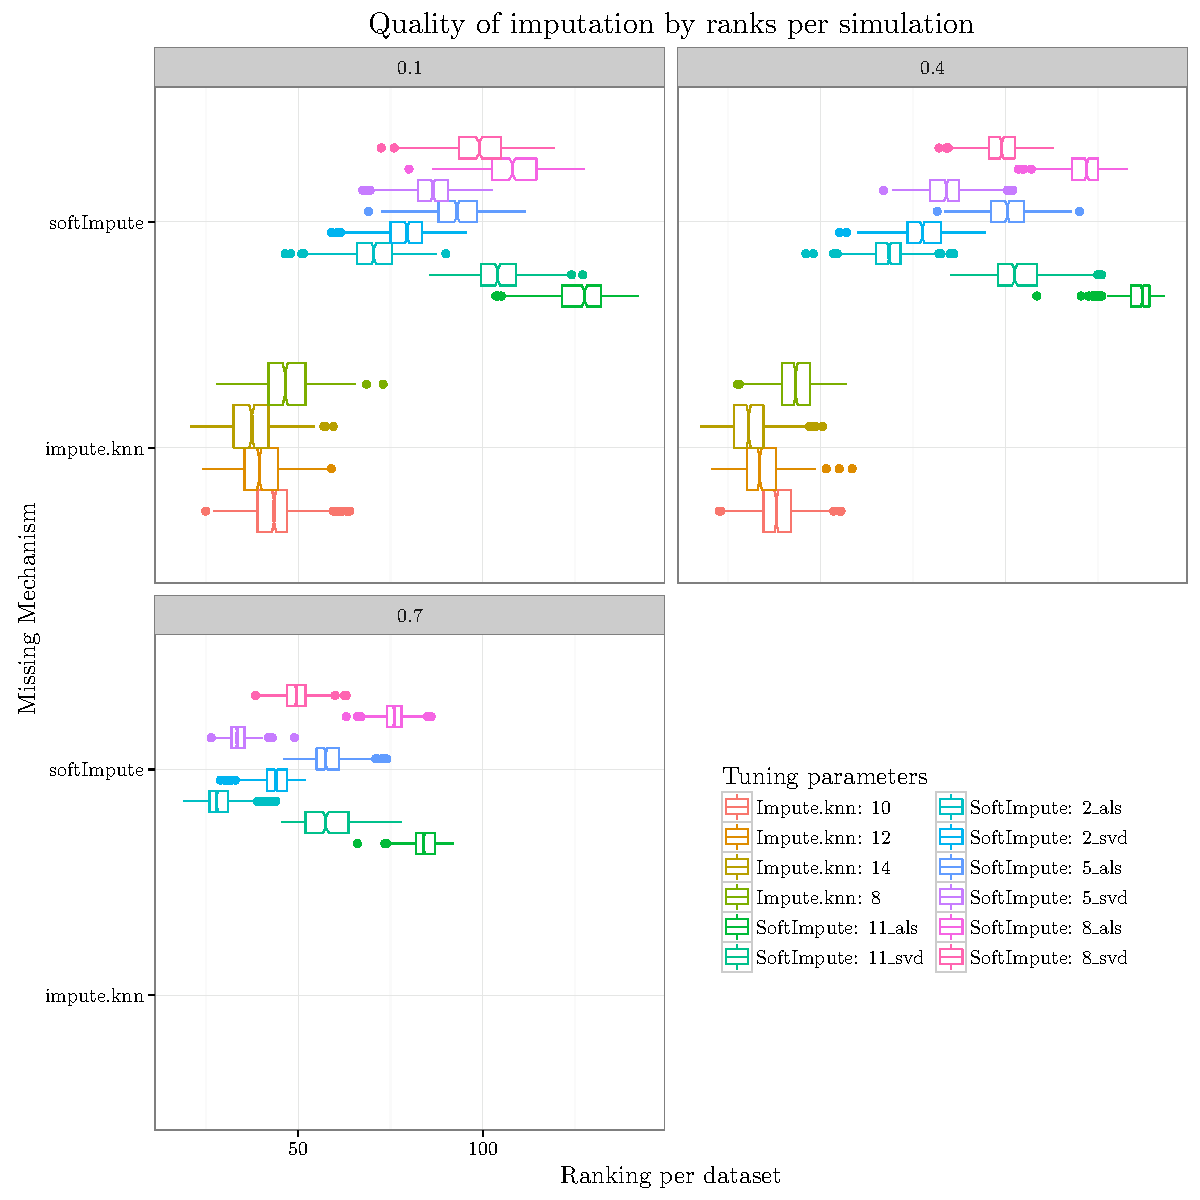
\includegraphics[width=\textwidth]{tuning_ranking_soft_impute_plot}
  \caption{Relative ranking of imputation quality of the tuning parameters of
    softImpute and impute.knn. For impute.knn, the number of neighbors is the
    tuning parameters, whereas for softimpute, it is the maximum rank and estimation
    method of the output matrix.}
  \label{fig:tuning:param:softimpute:imputeknn}
\end{figure}

\paragraph{Tuning parameters}
For the packages \texttt{softImpute} and \texttt{impute}, some defaults
parameters for the imputation methods are provided. Figure
\ref{fig:tuning:param:softimpute:imputeknn} displays how the quality of the
imputation evolves with the parameters. The \texttt{impute.knn} function, the
quality of the inference grows with the number of neighbors. The
\texttt{softImpute} function unexpectedly offers good default parameters, even
if some restrain should be kept when the missing rate is high.

\section{Results}

Figure \ref{fig:ranking:imputations} summarize the results under the
\textsc{mcar} missing mechanism. \texttt{softImpute} and \texttt{mice} were the
only package able to cope with a quite high missing rate ($p \geq
0.7$). \texttt{impute.knn} from the \texttt{impute} package, when it works, is
almost always the method with the best score, as defined in Equation
\eqref{eq:score:imputation}. \texttt{mice} offers a good balance between speed,
robustness and quality of imputations, but the methods depends on the linear
dependency of the columns of the data matrix. Although \texttt{softImpute} can
cope with almost any type of data matrix, its inferences are sub-par with the
other methods. Some further analysis might be needed to confirm this
results. \texttt{Amelia} is the package which is the least able to cope with a
random impute matrix: routines failed without exception with any missing rate
above $p > 0.3$. The \texttt{Amelia} and \texttt{mi} packages use by default
parallel back-ends to perform their computations. However, they are the slowest
methods in terms of elapsed time. This might be overcome by setting the number
of iteration to a lower threshold. Nonetheless, this is not recommended as
convergence is not guaranteed when data input might have dimensions with strong
linear dependency.

Figure \ref{fig:mse:mcar} shows the measure from Equation \eqref{eq:smse} for
missingness rates $p \in \{0.2, 0.5, 0.7\}$. For numerical data, all methods
but \texttt{softImpute} have the same order of errors with K-nearest neighbors
being slightly better than the others. However, the latter method does not
allow for inference of the imputation error.  As Figure \ref{fig:mse:mar}
shows, the previous statements are not impacted by changing the missingness
mechanism to (our implementation of) \textsc{mar}.

\section{Open questions}

Heuristically, the quality of models output normally depends on the amount of
available data. In the missing data framework, precision are needed for this
notion: Is it the number of complete observations, the number of non-missing
values, or a mixture of both?  Interactions between the number of observation
$n$, the number of dimensions $p$ and imputation methods with their optimal
parameters are left unanswered with this work. In order to answer this
question, a multivariate sampling mechanism should be devised and tested.

Moreover, are there any reasonable solutions which can be applied to overcome
collinearity? One could cluster the similar dimension and then pick one randomly
to create an imputed value. Nevertheless, such solutions were not yet
implemented.

Additionally, this small simulation study has been applied to certain data set
and it should be interesting to repeat the experience with other real data.

Finally, the concern of this work has been to apply imputation methods to
retrieve potential candidate values for inference, it would have been
interesting to verify the quality of inferences performed with the imputed data
set, for example multiple imputation against nearest neighbors.


\begin{figure}
  \centering
  % ../../R/output_analysis/output_analysis_partialdataset.R
  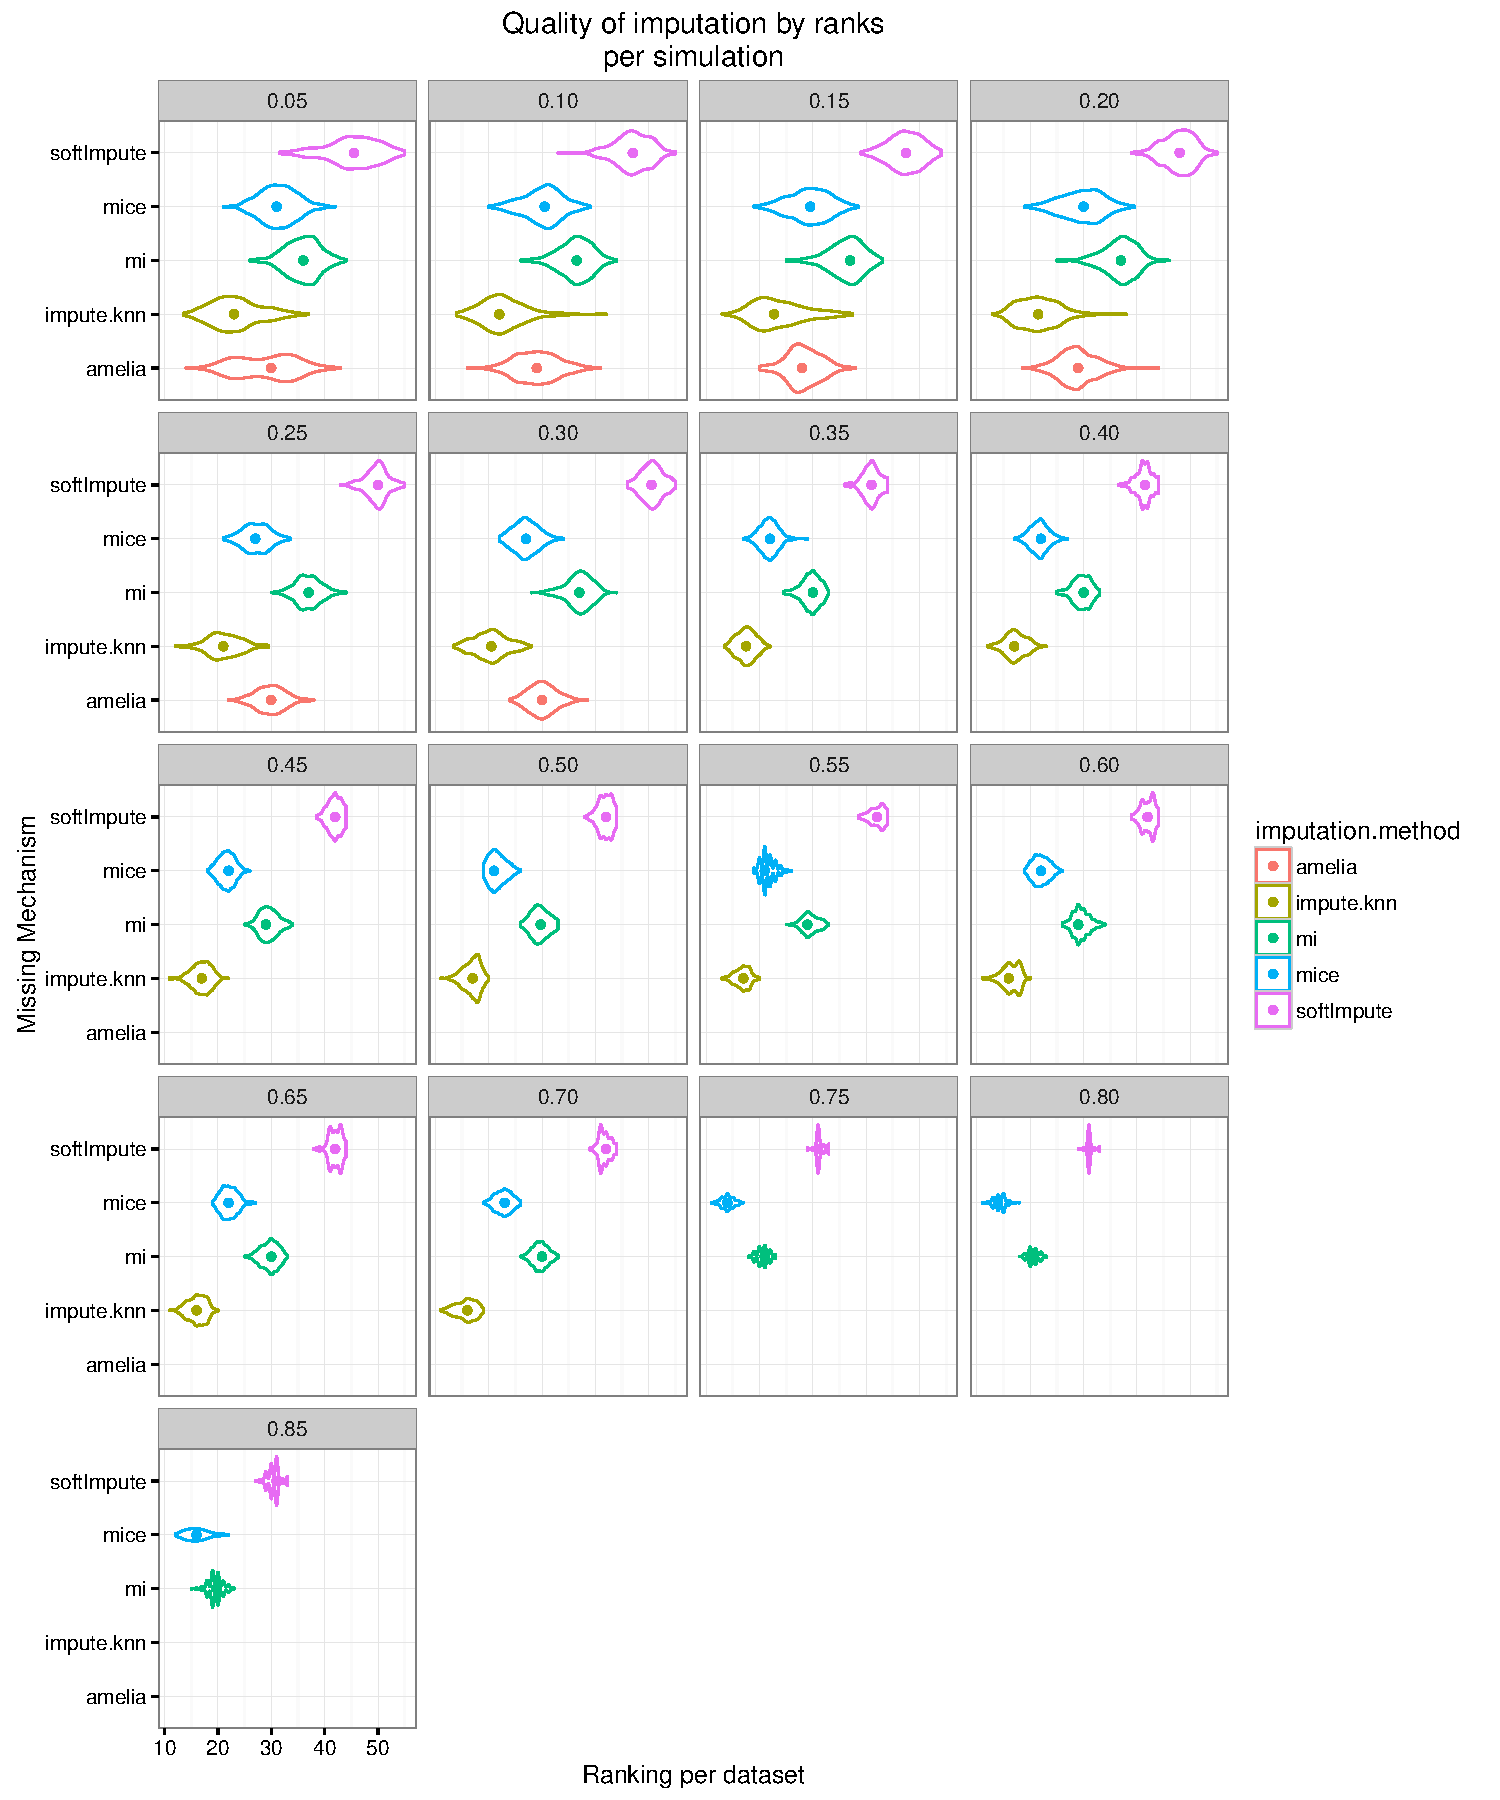
\includegraphics[width=\textwidth]{partial_ranking_plot}
  \caption{Rankings of imputation methods on the FLAS data set grouped by
    missing rate, under the MCAR mechanism with missing rate. Labels in the
    boxes provide the missing rate.}
  \label{fig:ranking:imputations}
\end{figure}


\begin{figure}
  \centering
  % ../../R/output_analysis/output_analysis_partialdataset.R
  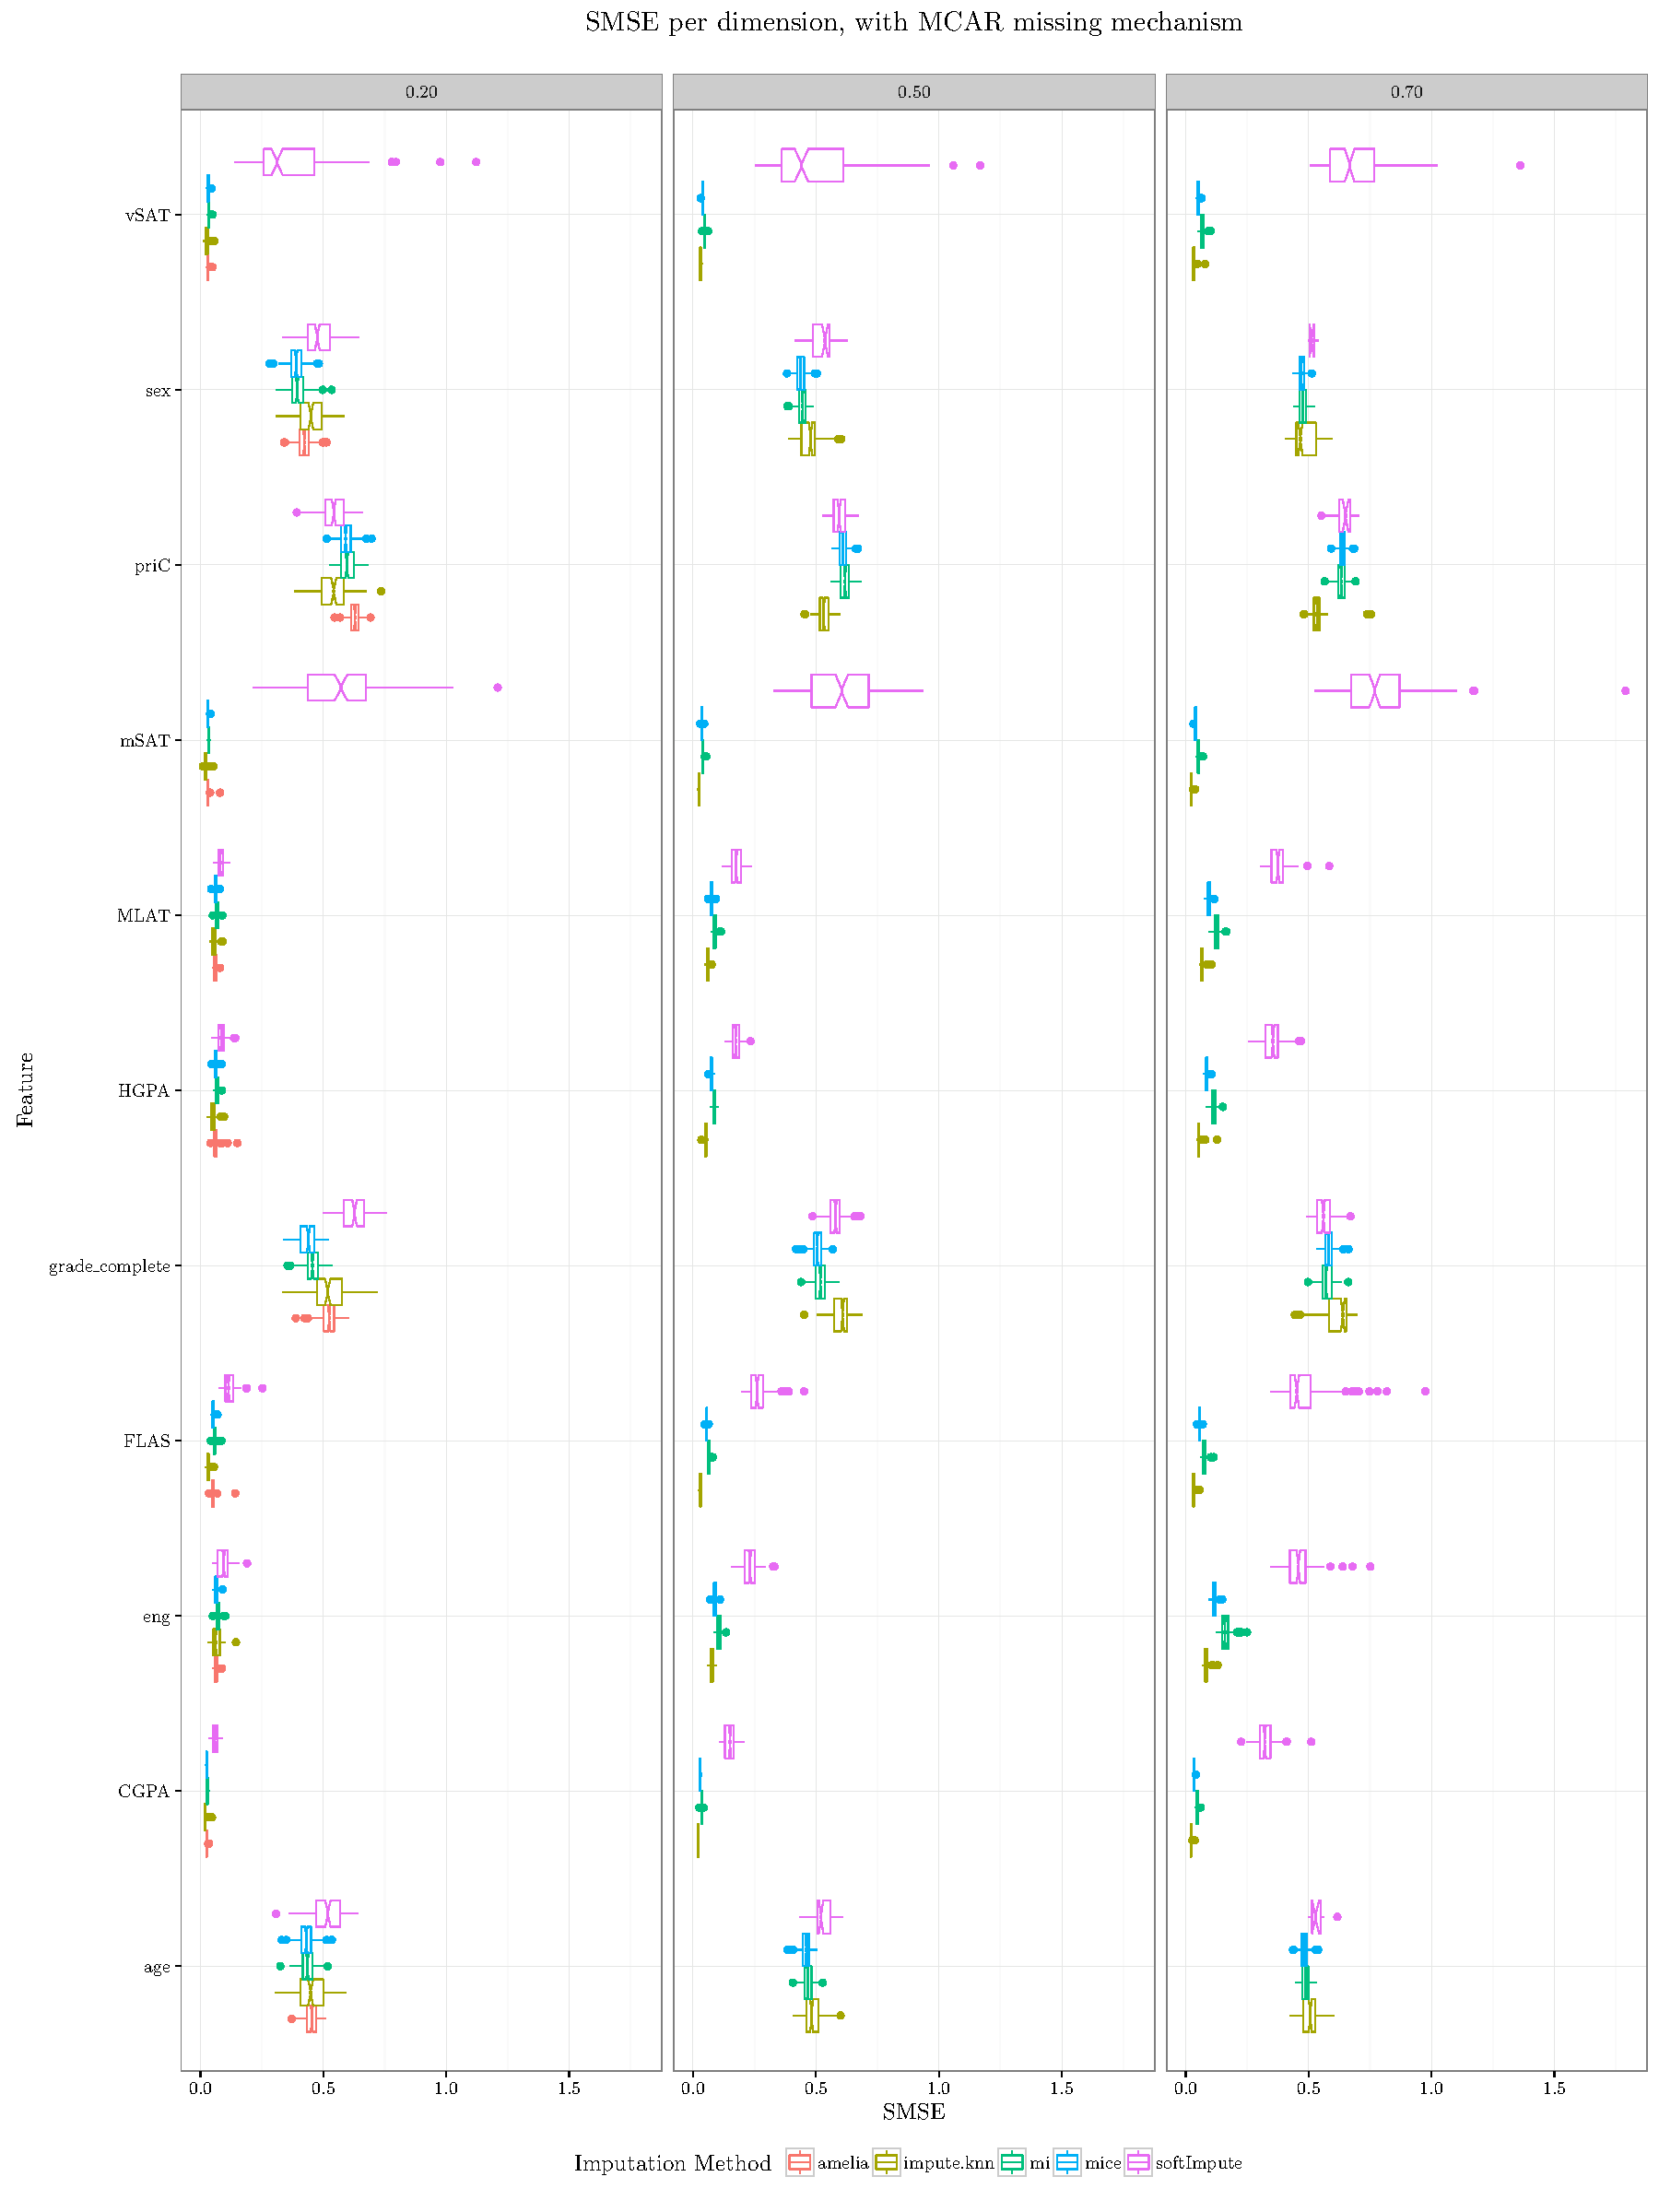
\includegraphics[width=\textwidth]{partial_mcar_measures_prob_selection}
  \caption{SMSE for selected missingness rate with MCAR
    against imputation methods.}
  \label{fig:mse:mcar}
\end{figure}


\begin{figure}
  \centering
  % ../../R/output_analysis/output_analysis_partialdataset.R
  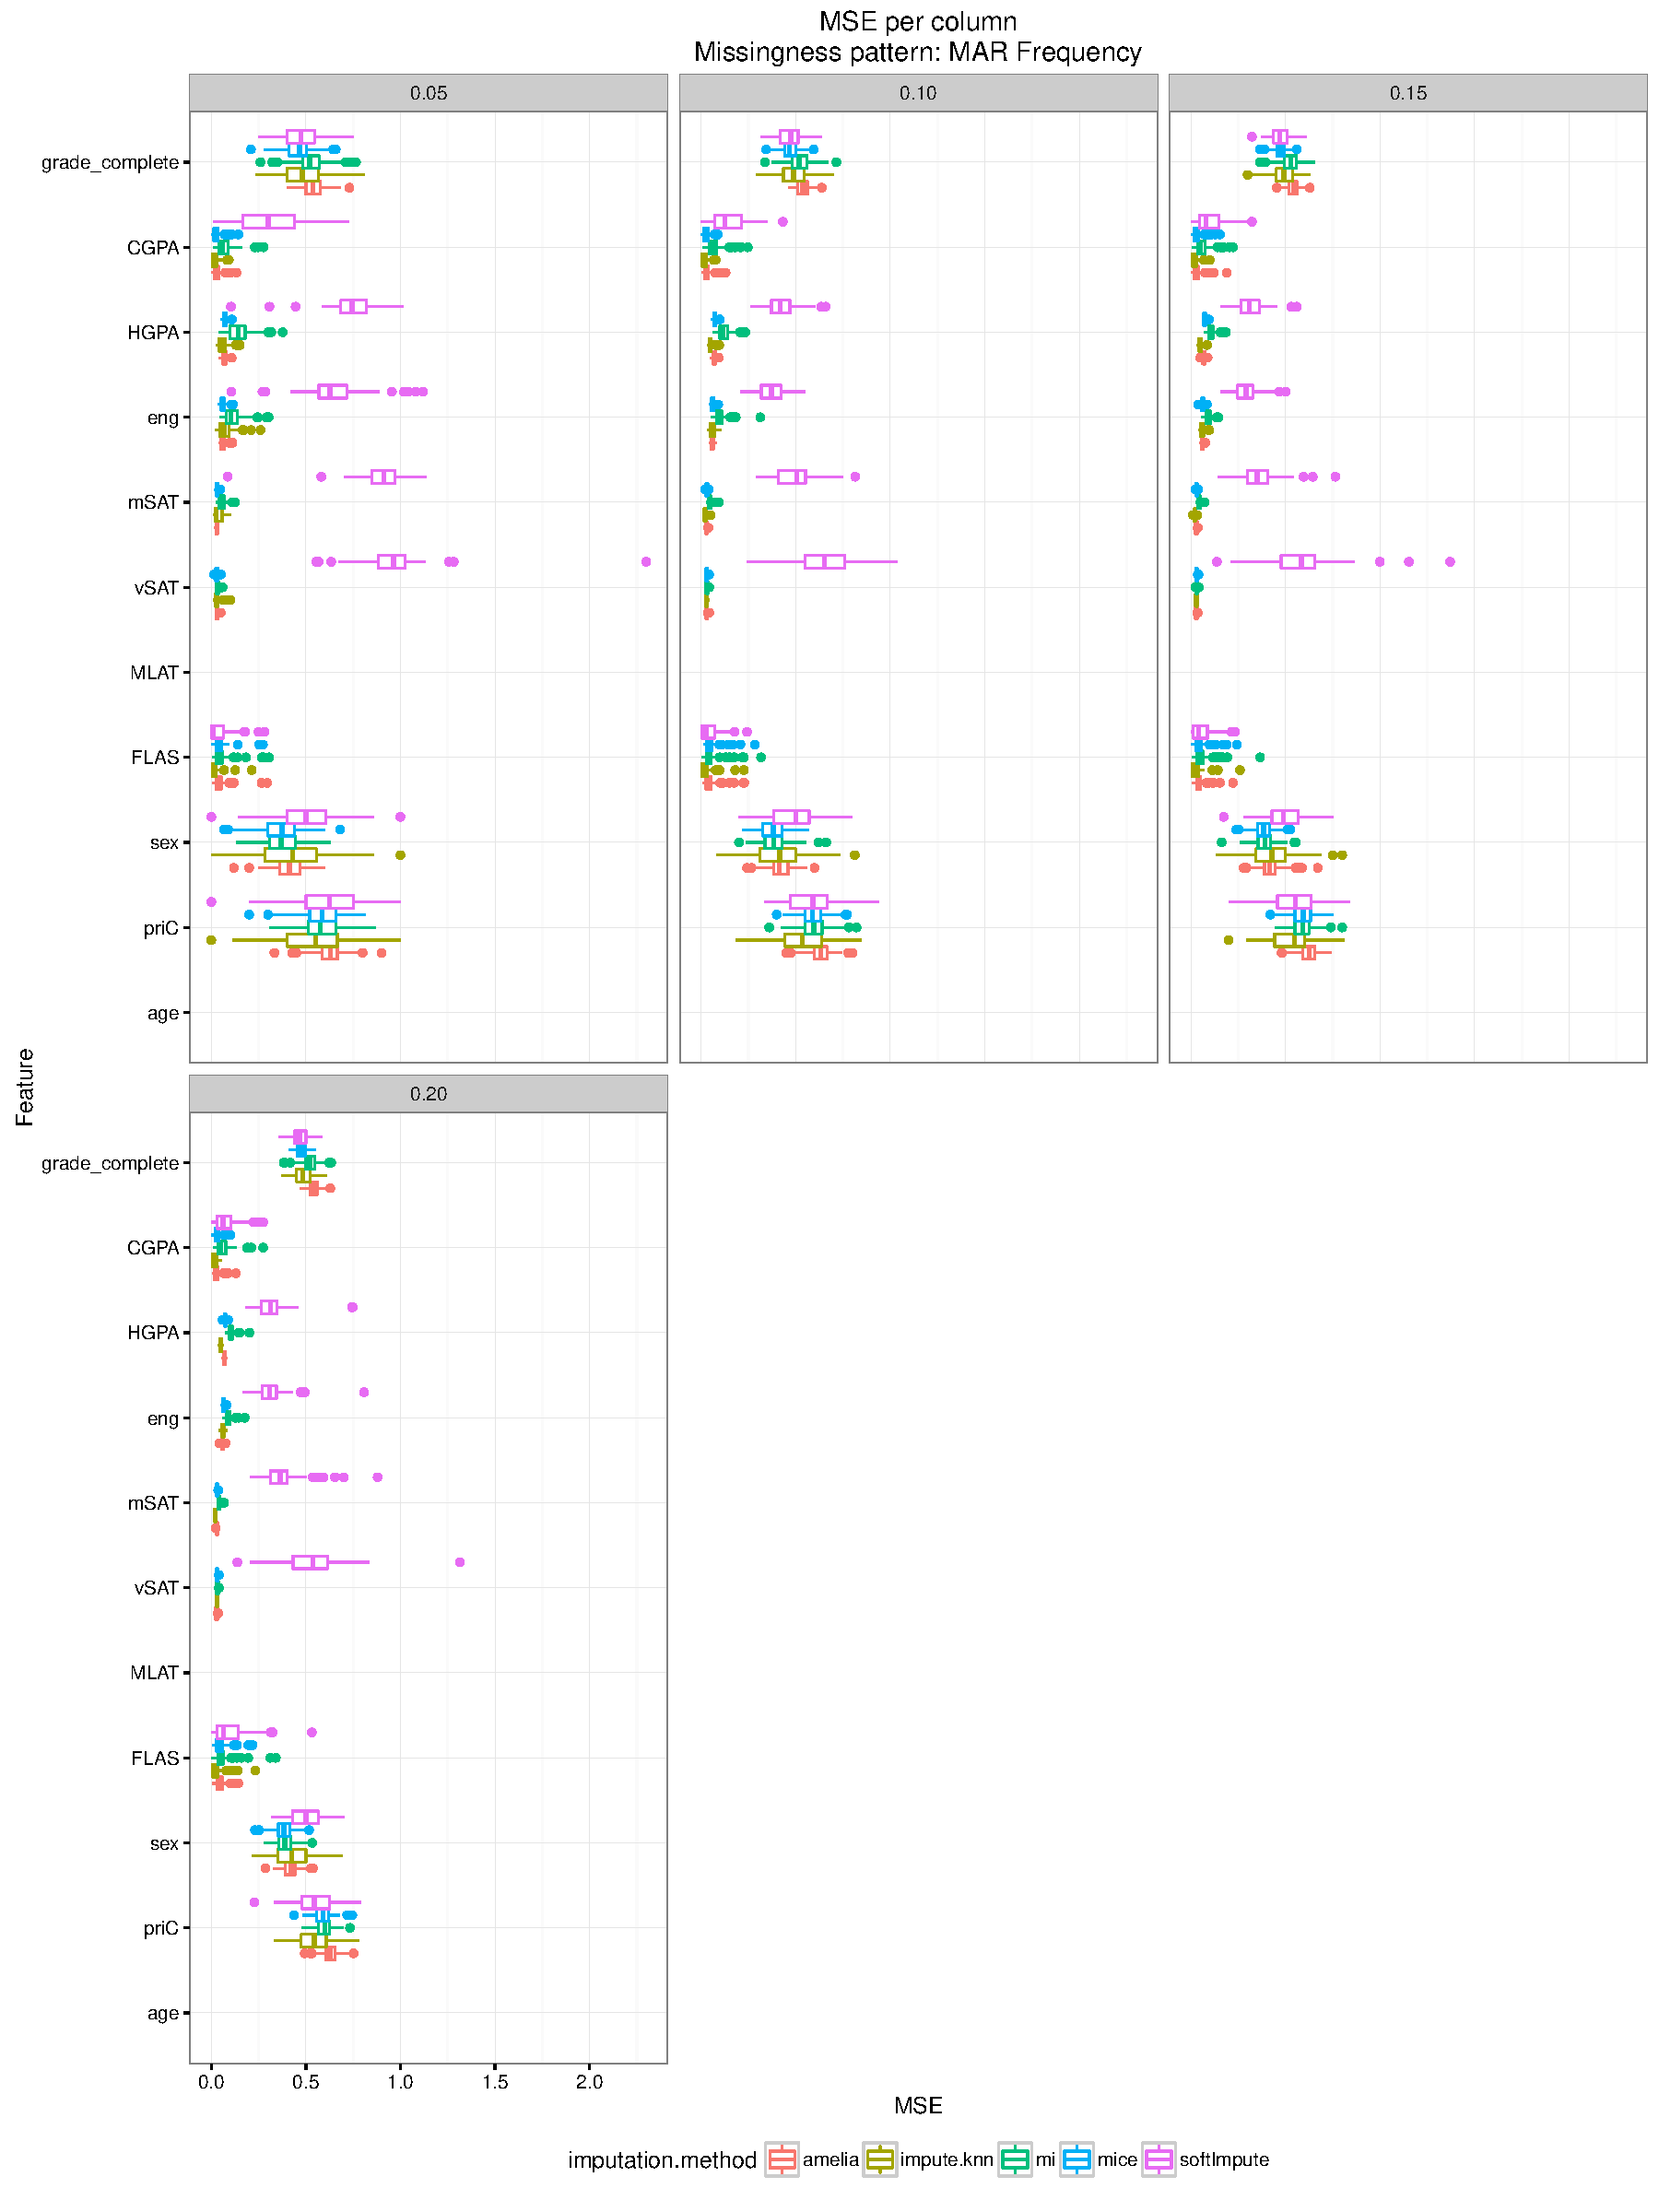
\includegraphics[width=\textwidth]{partial_marfrequency_measures}
  \caption{SMSE of imputation methods on the FLAS data set grouped by missing
    rate, under the MAR mechanism. Labels in the boxes provide the missing
    rate.}
  \label{fig:mse:mar}
\end{figure}



%%% Local Variables: ***
%%% mode:latex ***
%%% TeX-master: "semester_paper_sfs.tex"  ***
%%% End: ***
%%% reftex-default-bibliography: ("biblio.bib")
